\documentclass[a4paper]{article}

%% Language and font encodings
\usepackage[english]{babel}
\usepackage[utf8x]{inputenc}
\usepackage[T1]{fontenc}

%% Sets page size and margins
\usepackage[a4paper,top=3cm,bottom=2cm,left=3cm,right=3cm,marginparwidth=1.75cm]{geometry}

%% Useful packages
\usepackage{amsmath}
\usepackage{graphicx}
\usepackage[colorinlistoftodos]{todonotes}
\usepackage[colorlinks=true, allcolors=blue]{hyperref}

\title{The State of Voting Systems in the Twenty-First Century}
\author{Thomas E. Mason, Nisarg Patel, Inavamsi Enaganti \\ Advisor: Bud Mishra}

\begin{document}
\maketitle

% \begin{abstract}
% Your abstract.
% \end{abstract}

\section{Introduction}

Over the course of the Twentieth and early Twenty-First centuries democracy has gone from being a novel governmental system in peripheral regions of the West to spreading practically throughout the world, to the point where it is routinely discussed as being a universal aspiration for all human societies on earth. During its rapid advance, however, the societies governed by democratic polities have undergone enormous transformations that have changed almost every dimension of social and political life, and have led to a completely new conception of the proper role a democratic state should play in its citizens lives. A citizen of a Nineteenth century democracy would find many facets of modern democratic societies utterly foreign - their attitudes towards minorities, war, gender, taxes, welfare, policing; the way governments communicate with their citizens through announcements and media; the international relations between states.\\

Despite democracy's success, the history of the past two hundred years has provided ample evidence of the pitfalls that can be present in societies that aspire to democratization. Countries such as India or the United States, in spite of their democratic deficiencies, have still managed to sustain democracy successfully - the cases of Turkey, Germany, Russia, Venezuela, Japan, and others illustrate how fraught and unstable democracy can be. The vast complexities and challenges of modern political life notwithstanding, the political institutions of many of the world's largest democracies have their roots largely in the Nineteenth century or even in the republican systems of Classical Antiquity. The Constitution of the United States, for example, was designed in an Eighteenth century world for an agrarian, undeveloped society of 3 million inhabitants, but today continues to provide the political system of a global superpower of 320 million, a task for which it was certainly not originally designed.\\

A careful study of both the collapse of certain democratic systems and the chronic problems that have developed in others have yielded certain patterns. However, institutions in old and new democracies continue to be designed and run without patching the vulnerabilities that have been identified, which represents a clear threat to democratic systems around the world. What we propose is a systematic reevaluation of long-standing of voting systems, amounting to a modernization of democracy for the 21st Century. We propose and provide initial experimental simulation results to evaluate Quadratic Voting, the "Democracy 2.1" system, and Single Transferable Vote. We will also briefly touch on blockchain-based vote tallying and record keeping, and error-correcting mechanisms that show promise. 

\section{Common Vulnerabilities of Classical Voting Systems}

\subsection{Two-Party Systems}
Beginning in the 1950s with the work of French political scientist Maurice Duverger, there is a growing body of work asserting that under a diverse set of conditions, democratic systems tend to converge as varying rates to a stable equilibrium dominated by a two-party system. While this tends to be particularly extreme in "Winner Take All" or "First Past the Post" systems, it has been observed more weakly in other systems as well, with the United States and India being two famous instances. This results from the existence of a Nash equilibrium: although it would be in the common interest of the population for a broader set of parties to have a legitimate chance at power, each party has no realistic chance of winning by standing alone, leading to the formation of coalitions to compete for power. Although many of these coalitions may be conceived of as temporary in nature, informal factors such as the bureaucracies that grow up around them tend to solidify them into more rigid political blocs, thus cementing a two-party system in power.

\subsection{Electoral Fraud}
Joseph Stalin once remarked "The people who cast the votes decide nothing: the people who count the votes decide everything". He ought to have known how true those words were; voter fraud has been one of the most systemic problems plaguing democracies throughout human history. Dictators, oligarchs and strongmen make prolific use of rigged elections to shore up their authoritarian regimes behind a facade of electoral success (Egypt, Russia and Libya are particularly notorious examples of supposedly "multiparty" elections). Even stable democracies such as the United States have not been free from this problem (such as during the 1960 presidential election).

\subsection{Paradoxes, Old and New}
Democracy fundamentally requires a population that feels like their preferences are respected and considered fairly to sustain itself over the long term. However, even in the event that a clean and fair vote proceeds between multiple parties that have broken out of a two-party duopoly on power, this is still not always possible. Arrow's Impossibility Theorem and Condorcet Paradox illustrate this problem powerfully.
The Condorcet paradox states that collective preferences in a population can be cyclic and therefore non-transitive. For example, a majority can prefer candidate A to candidate B, and candidate B to candidate C, but not candidate A to candidate C. This can result, for example, in a perfectly free and fair election selecting deeply unpopular people over and over. An even stronger warning to democratic procedure comes in the form of Arrow's Impossibility Theorem, which states that it is impossible to transitively satisfy the will of a population without relying on a "dictator" to implement policies that the population wants but won't get given their current situation. However, more generally Arrow's Impossibility Theorem asserts that democratic systems will always have trade-offs between certain desired properties, and there is no "global optimum" system that maximizes all of them.\\

These two paradoxes can have grave implications for democracy: even if classical democratic systems are functioning "as designed", they can still frequently result in outcomes that are frustratingly unaligned with the desires of the majority of the population. This can, in the long run, foster mistrust and resentment toward democracy, and lead to an erosion of democratic participation. This can additionally lead to a vicious cycle, whereby democracies become even more moribund and dysfunctional, until the people turn to autocrats who offer simple solutions to their frustrations.

\subsection{Additional Chronic Problems}
A comprehensive list of issues facing voting procedures would be impossible to enumerate here, however there are still several commonly cited issues that bear discussion. The first of these is the Median Voter Theorem, which states that a vote should capture the "Median" preference of the electorate, sensibly enough. However, this is generally possible only when candidates can be ranked on a single-dimension scale, which is obviously not possible in any real world scenario, as there are many disjointed dimensions along which a candidate could define themselves. Political scientists have sometimes taken to defining candidates on a scale of being "right-wing" to "left-wing" although it has been noted by many political thinkers that even this simplistic rendering is not a useful distance metric in any meaningful sense. For example, how would an anti-immigrant, anti-clerical, environmentalist, socialist, pro-LGBT, isolationist candidate be ranked on a "right-to-left" spectrum? \\
Tactical voting is a second problem commonly cited in democracies. This essentially is where people cast their votes not for the "best" choice in their minds but the most realistic choice. This reality lends itself easily to crowdthink, where initial popularity of an idea or candidate plays an outsized role in whether it is ultimately selected. This has been hypothesized by Noam Chomsky and other political scientists to be highly deleterious to democracy, as it gives an electorate little actual power to dictate the country's policies, instead giving a choice between a highly curated "menu" of restricted options. Similarly, this can artificially narrow the range of possible solutions to a problem, which is one of the reasons why many electorates tend to converge over time to a two-party system. \\
Lastly, and also significant in the emergence and consolidation of two-party systems is the "Spoiler Effect" - where an unpopular candidate wins an election because two similar candidates split the vote between them, thereby losing (an example of this is Al Gore and Ralph Nader in 2000 in the US).

\section{Our Proposal}

\subsection{Error Correction Mechanisms}
%error correction Zipf's law - Libya example  -benford's law
There is a famous example of voter fraud that occurred in the late 2000's in Libya, where an election was held over the head of state, where the longtime dictator of the country Muammar Qaddafi won reelection. However, the election was highly suspected of being rigged. This suspicion was confirmed by an analysis by a team from MIT after the vote was concluded. Taking the least significant digit of the voting counts from each polling precinct, the distribution would be expected to be approximately evenly distributed. However, humans are notoriously bad at generating random numbers, which led the investigators to discover a highly non-uniform distribution of the least significant numbers. From this, the researchers concluded that the votes had been rigged, as the final counts were extremely unlikely to have resulted naturally. \\
Given the advancements that have been made in recent decades in random number generation and computing power, these error correcting mechanisms should absolutely be built into any voting scheme, and can be one of the enforcement conditions in the blockchain validator that maintains the vote ledger. Although this would not strictly eliminate vote stuffing, it would force malicious parties to be far more coordinated and sophisticated in their attacks and would leave far more room for detecting deceptive behavior.

\subsection{Blockchain}
Traditional democratic systems have functioned by relying on an election commission to collect, tabulate, and oversee the casting of votes. While there certainly exist tools to enforce fairness in this process, putting the calculation of election outcomes in the hands of a single organization is fundamentally an insecure method that is limited by the trust one can place in that organization. Even in democratic countries, federal and state election agencies are frequently accused of meddling or vote rigging, to say nothing of semi-democracies or democratizing countries. \\

To address this problem, we propose an approach inspired by blockchain smart-contracts (as illustrated in Figure 1). The concept underlying this would be to construct a signalling game between a Voter and an Electoral Commission, where deception in the signal is reduced by a Verifier or Miner, who performs one-way computationally hard problem. The mechanism would work by essentially making each vote cast be analogous to a transaction on a network like Bitcoin or Ethereum; the Voter would cast their vote, the Election Commission would receive their vote, and then non-strategic Miners would undertake a hard task to verify the vote had been cast correctly. Blockchain is well-adapted to this task, as elections are a discrete event that is by design supposed to be immutable, and can either be accepted as valid or rejected in its entirety. An interesting problem that this would prompt however is how to fairly distribute mining power in such an election. We propose that mining should be conducted by a government election commission. \\

An additional safety mechanism for this system would be to incorporate error-correction into the blockchain. Based on the tools enumerated above, a smart contract enforced over the voting blockchain would also have to meet the criteria needed to be random - if the votes cast indicated sufficiently non-random behavior to imply that fraud and tampering had occurred, the blockchain would revoke the contract and force the vote to be held again. This is significant because in practice many democratic countries have a problem with opting not to act even when widespread voter fraud is believed to have occurred - it is expensive and inconvenient to redo a vote and the party that wins has an incentive to insist the vote was fair. This system would eliminate this problem, although it could make elections more susceptible to denial-of-service attacks.
\begin{figure}[h!]
\centering
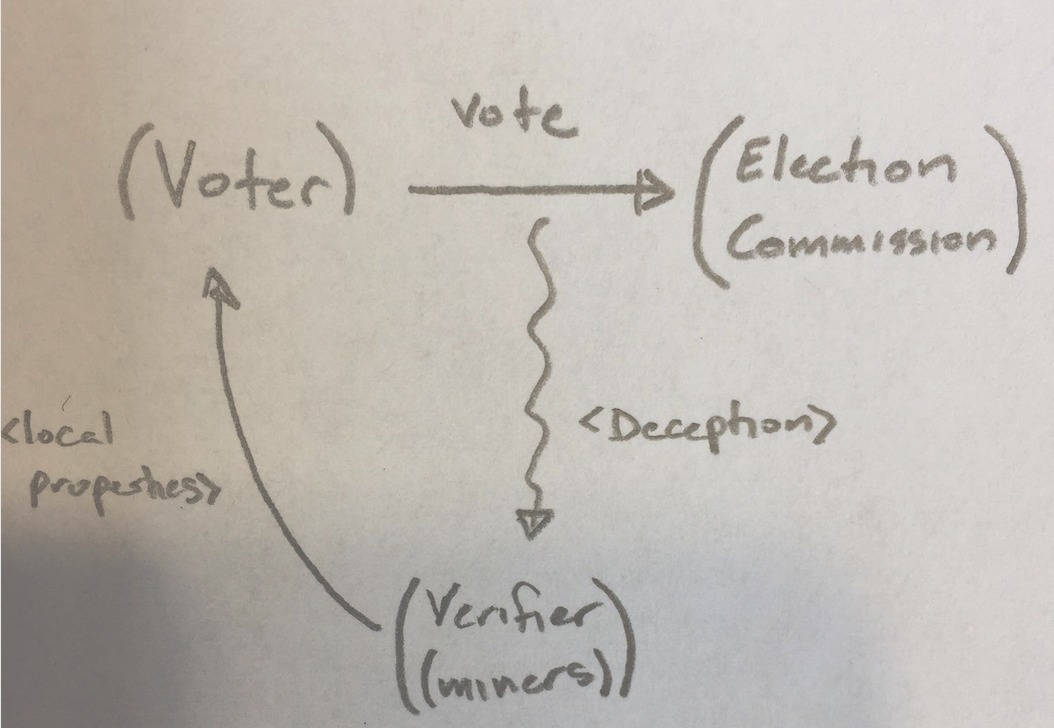
\includegraphics[width=45mm]{votechain.png}
\caption{A simple caption \label{overflow}}
\end{figure}

\subsection{Alternate Voting Procedures}
\begin{enumerate}
\item Single Transferable Vote
\item Democracy 2.1
\item Quadratic Voting

\end{enumerate}

We propose a model to combine the best merits of the above models in the methodology section. We have discussed a complete overhaul and a new system in the Discussion Section below.

\section{Methodology}

We have implemented a simple Python simulation to evaluate the following systems:
\begin{enumerate}
\item Preference Voting 
\item Negative Voting 
\item Random Selection 
\item Multiple voting 
\item Ensemble of above methods. 
\end{enumerate}

For the first 4 systems we have simulated elections on data sets and computed the values of the three metrics defined in the above Section. We have implemented an ensemble model to create an set of parameters that take into account the above 5 voting systems, as as to maximize the 3 Indexes for sample elections.
\\
\\
We have defined 3 metrics to gauge voting systems:
\begin{enumerate}
\item Threshold Index - Percentage of voters that are favourable to candidate
\item Acceptance index - Value determined by difference of Percentage of voters accepting candidate and Percentage of voters rejecting candidate
\item Match Index - How close is the result to the match to preferneces of population
\end{enumerate}

We have created a framework for a Supervised Learning Model using Simulated Annealing. 
Given a base system of rules A, we have to modify A so that it maximizes a certain fitness metric. We can calculate the value of the metric if we are given the winning candidates and the preferences of the voters. It is imperative that throughout the modifications the system should always make sense and should be explainable in human terms. Unlike Deep Learning where abstract parameters and states are generated, we have to ensure that the final voting system makes sense.

\section{Experimental Results}
\subsection{ Single County }
One County, 4 Candidates
\begin{center}
\begin{tabular}{ | c | c | c | c |c|  }
\hline
System & Victor &	Acceptance &	Threshold &	Match \\
	\hline
FPTP & 2 &	46.15 & 30.77 &	61.53 \\
\hline
Multiple & 3 &	76.92  &	53.84 &	26.92 \\
\hline
Preference & 1 &	53.84 & 30.77 &	46.15  \\
\hline

\end{tabular}
\end{center}

\subsection{ Two County }
We considered an election on two counties with the 5 same candidates standing for office in both counties.
\begin{center}
\begin{tabular}{ | c | c | c |c |c |c|  }
\hline
System &	Acceptance Index &	Threshold Index &	Match Index	& Victors	
 \\
\hline
FPTP &	51.28 &	30.77 &	51.28 &	2, 2  \\
\hline 
Multiple &	62.82 &	41.02 &	35.89 &	3, 4  \\
\hline
Negative &	64.10 &	30.77 &	23.07 &	1, 1 \\
\hline
Preference &	51.28 &	30.77 &	48.72 &	2, 4  \\
\hline

\end{tabular}
\end{center}

\subsection{ Ensemble Model }
We considered an election on two counties with the 5 same candidates standing for office in both counties.
\begin{center}
\begin{tabular}{ | c | c | c |c |c |c|  }
\hline
System & Total Score \\
\hline
FPTP &		133.33 \\
\hline 
Multiple &		139.73 \\
\hline
Negative &		117.94 \\
\hline
Preference &	130.77 \\
\hline
Ensemble & 150.3 \\
\hline

\end{tabular}
\end{center}

% Basic Experiments \dots
% \dots or bullet points \dots
% \begin{itemize}
% \item Like this,
% \item and like this.
% \end{itemize}

\section{Discussion and Future Research}

We will discuss a completely new voting system. Before that we will run through a few interesting instances that will help verify and consolidate the idea.\\

 One interesting case study is that of the crowdsourced "Twitch plays Pokemon" game from several years ago. Twitch plays Pokemon is a social experiment on an online platform using a poll for every move made in the game. The experiment was carried out on a complicated Pokemon Red Game in a free world with multiple attributes. The game had over 16 days of game play and over 1.2 million unique players participating in the polls. Every action of the main character during the game was crowd-sourced using a poll. Although the end goal of the game was clear, locally there were a huge number of varied and most of the time contradicting strategies. With only 8 input option there were 1000's of possible actions the character carried out based on the situation he was in. From solving complex puzzles to combating people dedicated to spoil the game, the game successfully concluded within 17 days where the average time is 27 hours and a rushed average of 17 hours. \\ \\
The following system is an idea proposed for smaller controlled setting like a shareholder's meeting. When it comes to a government voting policy, a lot more consideration is required. \\

One obvious method would be to use a Deep neural network to obtaina  hidden funcion that correctly maps voter preferences. But it is imperative that throughout the modifications the system should always make sense and should be explainable in human terms. System should be very simple (Occam’s razor). \\

Before we discuss the new Voting system let us learn what we mean by constraints on the system. We use a bunch of inviolable constraints during construction of our voting system. These constraints are properties we would expect the system to enforce and it is done by maintaining them throughout the construction. \\ 



Example set of constraints:
\begin{enumerate}
\item Everyone is equal in elections for representatives. A person who didn't complete high school has the same say in matters of healthcare as somebody who holds an advanced degree in public policy when it comes to choosing a representative.
\item Every person is weighted according to educational qualification. (Ex : PhD in Science will have 20\% more weight-age than a high school dropout in matters related to Science policy).
\item If  less than 50 percent don't want someone to lead the country they cannot.
\item Candidate should rank in top 3 where total unhappiness is minimized.
\item Re-vote if p(election unfair) < k
\item Log rule : log of support is considered as opposed to direct support. The rest of support takes into account international forums, trade unions and other organizations.
\end{enumerate}

\\
We assume a decentralized system preferably on the block-chain. Right now we shall assume one time voting for a given period. This model can easily be extended to a dynamic system with the help of the decentralization and smart phones. \\
As opposed to traditional voting methods each voter writes up a set of contracts and these will be explained further. On a simpler setting each voter just has to fill out a survey as opposed to just naming one or many candidates.

So a simple contract could look like one of the following.
\begin{enumerate}
\item I endorse a candidate for the entire period of the term.
\item My vote is for candidate A unless there is a scam of Type A validated by the courts, then my vote belongs to B.
\item I am fine with either A or B and in the case of post-election alliance, withdraw support from candidate who allies with C. 
\end{enumerate} \\
Accountability is enforced. These contracts do have a lot of problems including instability for the government, and if we take it one step further in the case of the Brexit referendum it can be argues that the common man doe snot know what he wants. As stated before we will restrict the current discussion to controlled environment like shareholder meetings with easy to see end goal and simpler dynamics.
Also the representative can dynamically view rating and can predict which actions to do and not do to either not lose support or gain additional support. Al-though this will open up a whole new world of paradoxes and dirty-politics, certain rules can be enforced. 

We propose a comprehensive contract system which will extend into matters of concern that can enable authority to someone or something else. For example, if my aim is to keep jobs in the company and not outsource them, I will give my authority to agency of advanced studies in job analysis. This implies that relevant agencies will have to release manifestos and portfolios with respect to the election in question.

Now we get to the main system which involves aggregating all the constraints, voter contracts and all the information and evolves. The important thing is that contracts involves the rules of voting and also the metrics explained in the third section of the proposal. So in a way we purpose a rule evolving system that is completely created by the people. It could involve direct voting on certain policies and instances of the system but also allow other authorities to take over if allowed but the aggregated system. 

The main point of the system is that everything is decentralized and has a chance of being reset and changed. From the very concept of having contracts, to the the existence of constraints and the very notion of aggregating and evolving, all this should be given to the people. The sad truth is that people are stupid, but with the help of evolution and a long period of virtual simulation in parallel with the real government, it can be deployed after years of tempering. \\
Foreseeable problems with the system
\begin{enumerate}
\item Need a proper set of axioms so that the system is not stuck in a Nash equilibrium. 
\item Constraint set involves a forced reset in the case of an occurrence of an Abilene Paradox.
\item A proper fail-safe system in case of contract misuse or loophole
\end{enumerate}

\bibliographystyle{alpha}
\bibliography{sample}
\cite{saari}
\cite{chomsky}
\cite{duverger}
%\url{https://www.springer.com/us/book/9783540600640} \\
%\url{https://en.wikipedia.org/wiki/Tactical_voting} \\
%\url{http://www.mathcircles.org/wp-content/uploads/2017/10/VoteBeamer-1.pdf} \\
%\url{https://docs.google.com/forms/d/1VQoo0kKYNCFsc7nwV-XLR0FkkmCMW4uvainB95Vs5co/edit#responses} \\
%\url{https://en.wikipedia.org/wiki/Twitch_Plays_Pokemon} \\
%\url{https://www.wired.com/story/colorado-quadratic-voting-experiment/?utm_source=pocket-newtab} \\
\end{document}